\documentclass{beamer}
\let\vec\mathbf
\mode<presentation>
\usepackage{amsmath}
\usepackage{amssymb}
%\usepackage{advdate}
\usepackage{adjustbox}
%\usepackage{subcaption}
\usepackage{enumitem}
\usepackage{multicol}
\usepackage{mathtools}
\usepackage{listings}
\usepackage{url}
\usetheme{Boadilla}
\usecolortheme{lily}
\setbeamertemplate{footline}
{
  \leavevmode%
  \hbox{%
  \begin{beamercolorbox}[wd=\paperwidth,ht=2.25ex,dp=1ex,right]{author in head/foot}%
    \insertframenumber{} / \inserttotalframenumber\hspace*{2ex} 
  \end{beamercolorbox}}%
  \vskip0pt%
}
\setbeamertemplate{navigation symbols}{}
\providecommand{\nCr}[2]{\,^{#1}C_{#2}} % nCr
\providecommand{\nPr}[2]{\,^{#1}P_{#2}} % nPr
\providecommand{\mbf}{\mathbf}
\providecommand{\pr}[1]{\ensuremath{\Pr\left(#1\right)}}
\providecommand{\qfunc}[1]{\ensuremath{Q\left(#1\right)}}
\providecommand{\sbrak}[1]{\ensuremath{{}\left[#1\right]}}
\providecommand{\lsbrak}[1]{\ensuremath{{}\left[#1\right.}}
\providecommand{\rsbrak}[1]{\ensuremath{{}\left.#1\right]}}
\providecommand{\brak}[1]{\ensuremath{\left(#1\right)}}
\providecommand{\lbrak}[1]{\ensuremath{\left(#1\right.}}
\providecommand{\rbrak}[1]{\ensuremath{\left.#1\right)}}
\providecommand{\cbrak}[1]{\ensuremath{\left\{#1\right\}}}
\providecommand{\lcbrak}[1]{\ensuremath{\left\{#1\right.}}
\providecommand{\rcbrak}[1]{\ensuremath{\left.#1\right\}}}
\theoremstyle{remark}
\newtheorem{rem}{Remark}
\newcommand{\sgn}{\mathop{\mathrm{sgn}}}

\providecommand{\res}[1]{\Res\displaylimits_{#1}} 
\providecommand{\norm}[1]{\left\lVert#1\right\rVert}
\providecommand{\mtx}[1]{\mathbf{#1}}
\providecommand{\abs}[1]{\left\vert#1\right\vert}
\providecommand{\fourier}{\overset{\mathcal{F}}{ \rightleftharpoons}}
%\providecommand{\hilbert}{\overset{\mathcal{H}}{ \rightleftharpoons}}
\providecommand{\system}{\overset{\mathcal{H}}{ \longleftrightarrow}}
	%\newcommand{\solution}[2]{\textbf{Solution:}{#1}}
%\newcommand{\solution}{\noindent \textbf{Solution: }}align
\providecommand{\dec}[2]{\ensuremath{\overset{#1}{\underset{#2}{\gtrless}}}}
\newcommand{\myvec}[1]{\ensuremath{\begin{pmatrix}#1\end{pmatrix}}}

\title{Matrices in Geometry - 4.11.15}
\author{EE25BTECH11037  Divyansh}
\date{Sept, 2025}

\begin{document}

\maketitle


\section{Problem}
\begin{frame}
\frametitle{Problem Statement}
Find the equation of the plane which contains the line of intersection of the planes $\vec{r}\cdot\brak{ \hat{i}+2\hat{j} +3\hat{k}}-4=0$, $\vec{r}\cdot \brak{2\hat{i} + \hat{j} - \hat{k}} + 5 = 0$ and which is perpendicular to the plane $\vec{r}\cdot\brak{5\hat{i} +3\hat{j} - 6\hat{k}} +8 = 0.$
\end{frame}

\section{Solution}
\begin{frame}{Solution}
   
We need to find an equation of the plane that contains the line of intersection of the given two planes: 
\begin{align}
\vec{P_1}\  : \ \vec{n_1}^{\top}\vec{x}-4=0 \ \ , \vec{n_1}=\myvec{1 \\ 2 \\ 3 } \\
\vec{P_2} \ : \ \vec{n_2}^{\top}\vec{x}+5=0 \ \ , \vec{n_2}=\myvec{2 \\ 1 \\ -1 }
\end{align}
Another plane that passes through the intersection of these two planes is
\begin{align}
    \vec{P} \ : \ \vec{P_1} + \lambda\vec{P_2}=0 \\ 
    \vec{P} \ : \ \vec{n_1}^{\top}\vec{x}-4 + \lambda\brak{\vec{n_2}^{\top}\vec{x}+5}=0
\end{align}
\end{frame}

\begin{frame}{Solution}
This can be written as 
\begin{align}
    \vec{P} \ : \ \brak{\vec{n_1}^{\top}+ \lambda\vec{n_2}^{\top}}\vec{x} -4 + 5\lambda=0
\end{align}
The normal to this plane is 
\begin{align}
    \vec{n}=\vec{n_1} + \lambda\vec{n_2}
\end{align}

The plane $\vec{P}$ should also be perpendicular to the plane 
\begin{align}
    \vec{P_3} \ : \ \vec{n_3}^{\top} \vec{x}+8=0 \ , \ \vec{n_3}=\myvec{5 \\ 3 \\ -6} \\
    \therefore \vec{n_3}^{\top} \vec{n}=0 \implies \vec{n_3}^{\top}\brak{\vec{n_1} + \lambda\vec{n_2}}=0 \\
    \implies \vec{n_3}^{\top}\vec{n_1} + \lambda\vec{n_3}^{\top}\vec{n_2}=0
\end{align}
\end{frame}
\begin{frame}{Solution}
    \begin{align}
        \implies \myvec{5 & 3 & -6}\myvec{1 \\ 2 \\ 3 }  +  \lambda\myvec{5 & 3 & -6}\myvec{2 \\ 1 \\ -1 }=0 \\
    \implies -7 +19\lambda=0 \implies \lambda = \dfrac{7}{19}
    \end{align}
    Substituting this value of $\lambda$ in equation of $\vec{P}$, we get
\begin{align}
    \vec{P}\ :\ \brak{\myvec{1 & 2 & 3 } + \frac{7}{19}\myvec{2 & 1 & -1 }}\vec{x} -4 + \frac{35}{19}=0\\
    \vec{P} \ : \vec{n}^{\top}\vec{x}-41=0 \ , \ \vec{n}=\myvec{33 \\ 45 \\ 50}
\end{align}
\end{frame}
\begin{frame}{Solution}
\begin{figure}[H]
    \centering
    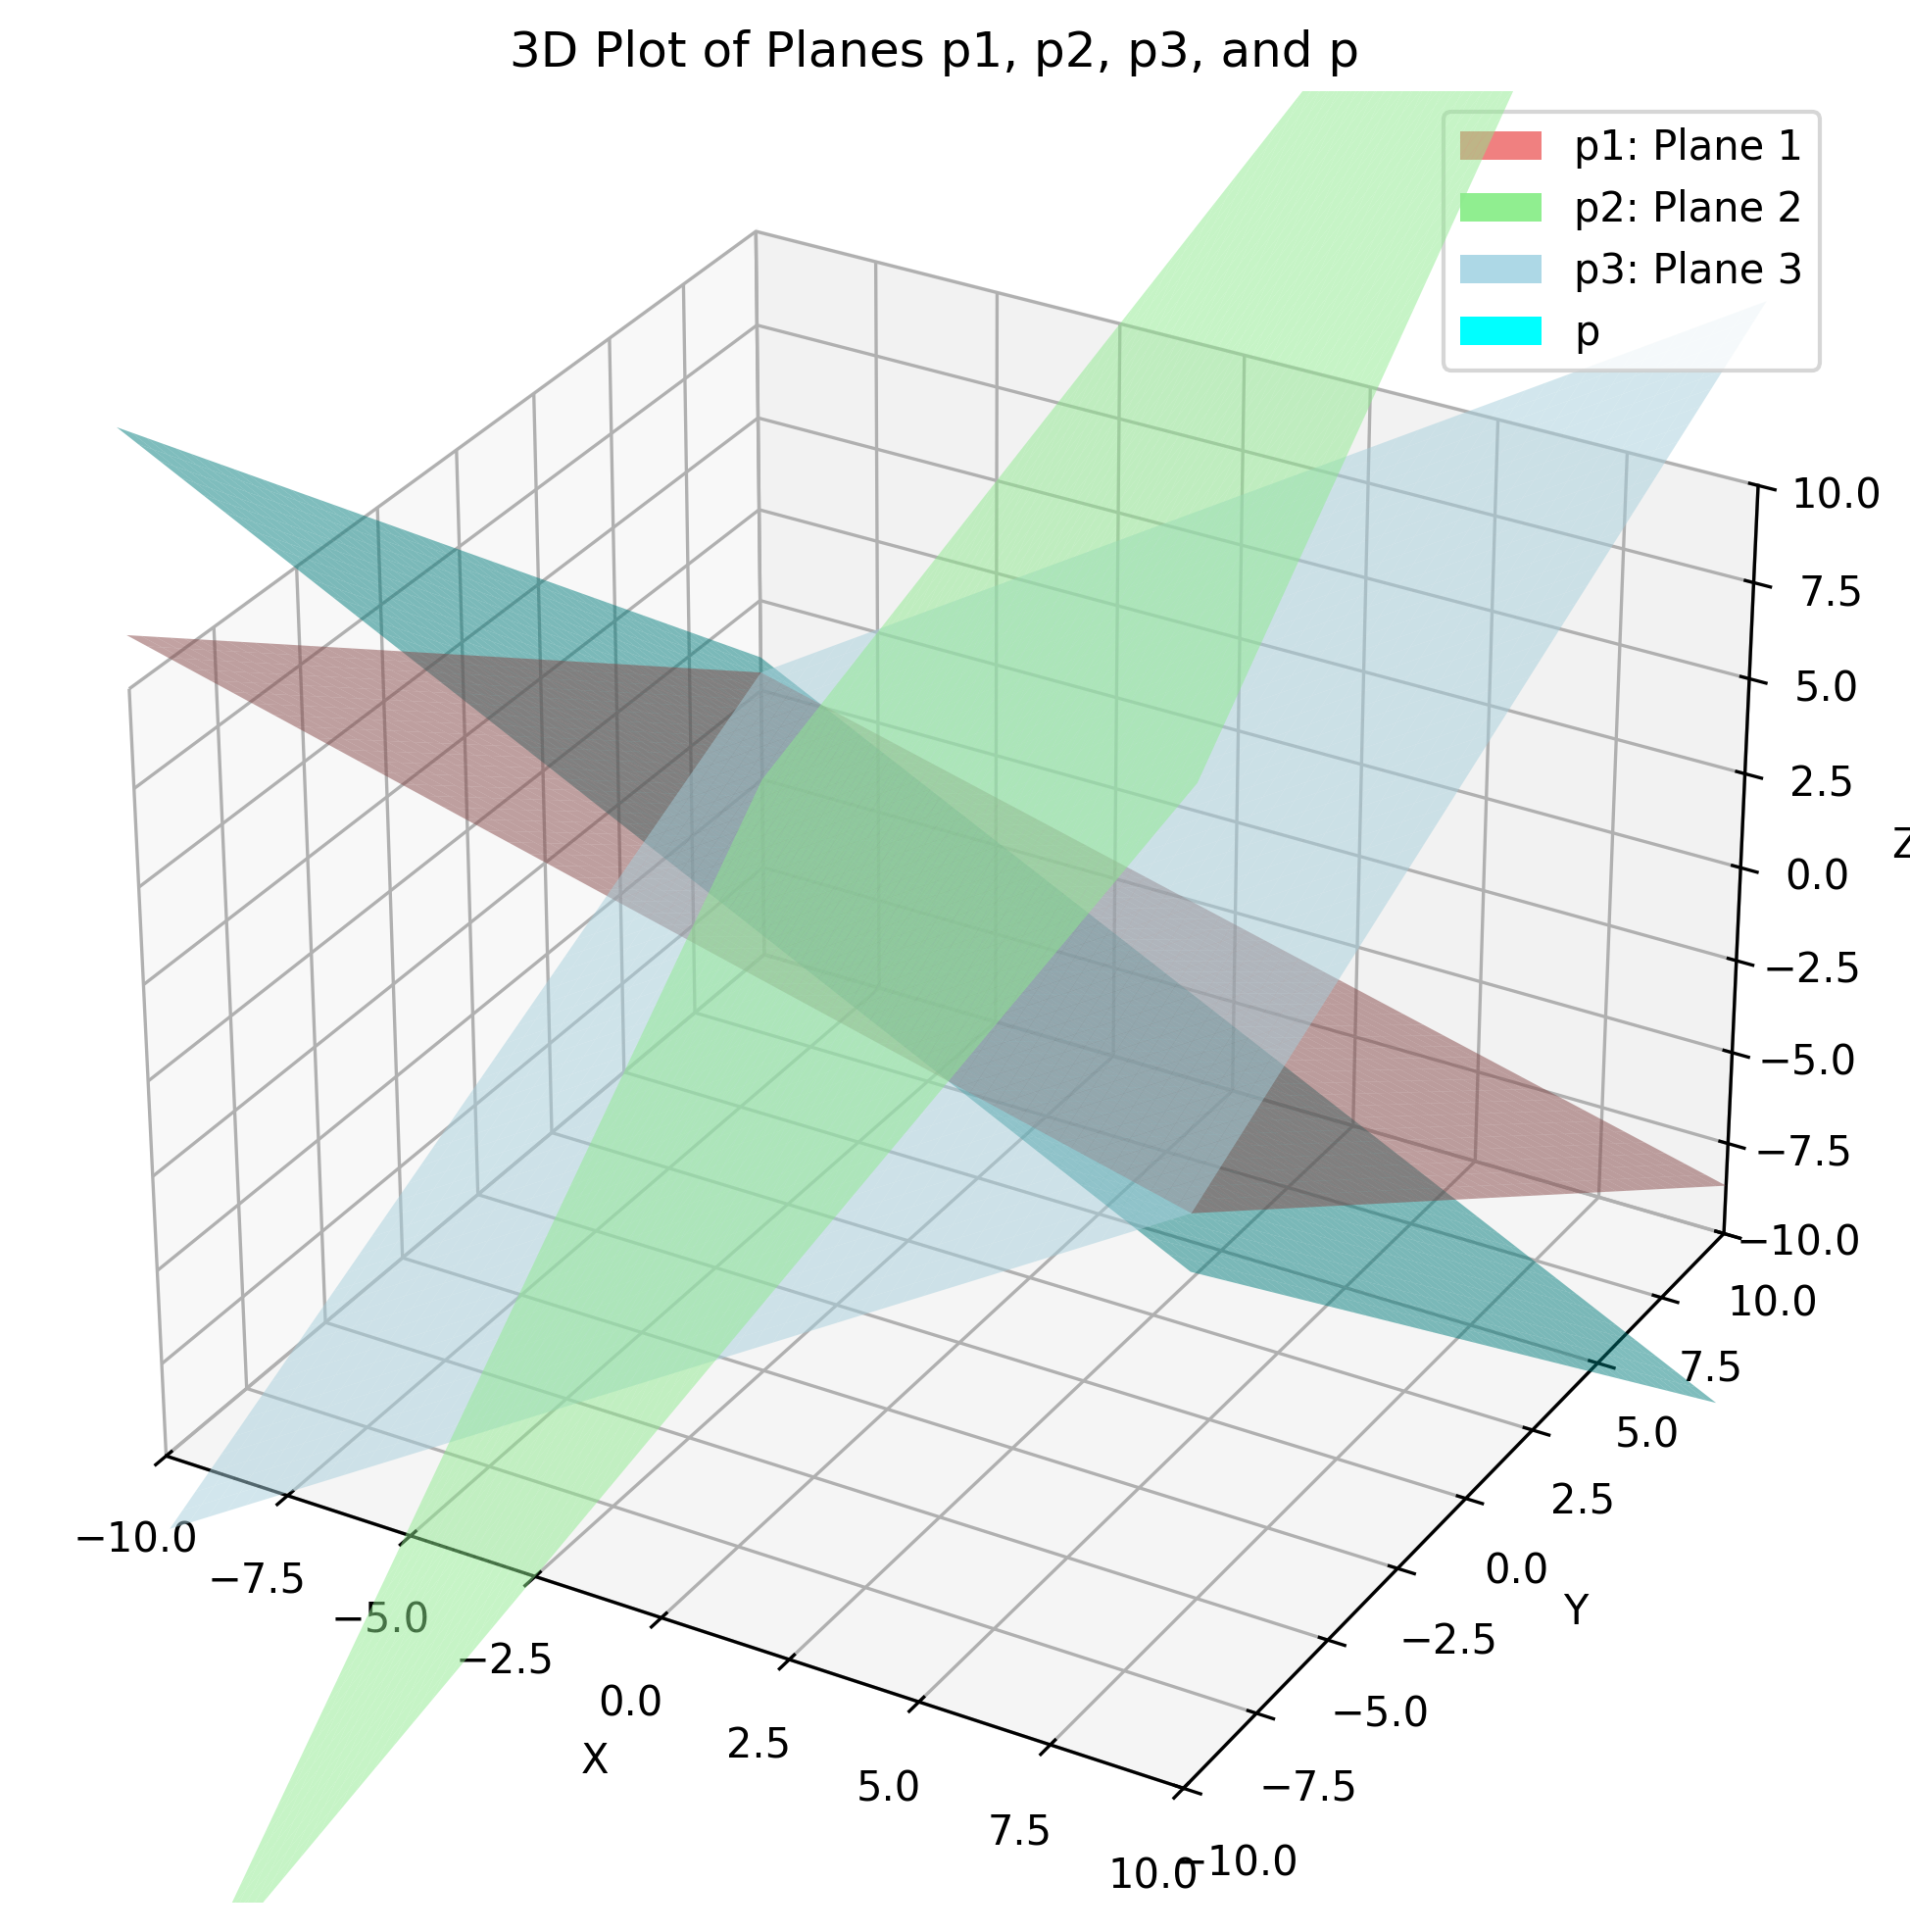
\includegraphics[width=0.5\columnwidth]{figs/1.png}
    \caption{Figure for 4.11.15}
    \label{fig:placeholder}
\end{figure}
\end{frame}


\end{document}
